% !TEX encoding = UTF-8
% !TEX TS-program = pdflatex
% !TEX root = ../tesi.tex

%**************************************************************
\chapter{Progettazione e realizzazione}
\label{cap:progettazione-realizzazione}
%**************************************************************

% \intro{Breve introduzione al capitolo}

%**************************************************************

\section{Progettazione}
Una volta completato lo studio e analizzato in dettaglio le tecnologie scelte abbiamo proseguito verso la progettazione
delle nostre componenti. Di seguito presenterò in sintesi come sono state modellate tutte le varie parti
dell'applicazione, divise per funzionalità.
\subsection{Login}

\begin{wrapfigure}{l}{0.5\textwidth}
  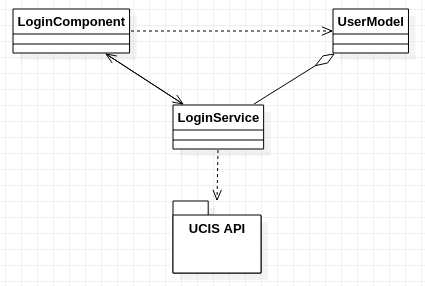
\includegraphics[width=0.9\linewidth]{login} 
  \caption{Diagramma login semplificato}
  \label{fig:login}
\end{wrapfigure}

La prima parte dell'applicazione della quale ci siamo occupati è quella di login. Per fare questo abbiamo optato per una semplice \acrlong{mvc}, con
una classe \textit{User} come modello, che rappresenta le informazioni di un utente, una \textit{View} composta da un semplice form con un
template Angular e un \textit{controller} che si occupa di contattare il server e mantenere l'utente autenticato gestito da un
\textit{service}. \\
\subsection{Struttura delle API del gestionale UCIS}

Le \gls{api} esistenti mettono a disposizione quattro tipi di richiesta:

\begin{itemize}
  \item l'autenticazione avviene tramite il metodo POST, dove nel body è inserita la username e la password. Il
  risultato ritorna la chiave, utilizzabile nelle richieste future. In caso le credenziali siano sbagliate ritornerà una
  pagina HTML con il seguente errore:

  \begin{lstlisting}[language=HTML]
    <div id="errorboxheader">0 - Class &#039;APIUnauthorisedException&#039; not found</div>
  \end{lstlisting}
  \item è possibile con una richiesta GET richiedere la lista delle attività di un utente. La risposta contiene una
  classe JSON con la struttura delle categorie e lista delle attività. 
  \item tramite richiesta PUT è possibile creare una nuova attività sul server associata all'account. Il client dovrà
  inviare la data in cui è stata creata l'id corrispondente alla categoria e l'id del cane con cui partecipa. Il server
  restituirà il codice associato all'attività.
  \item la gestione della registrazione avviene tramite richieste POST, nelle quali si specifica se sono di tipo
  \textit{start}, \textit{pause}, \textit{end} e \textit{log}. Ognuno di essi deve inviare al server la posizione e
  rispettivamente indicheranno se l'attività e ricominciata, è in pausa, è terminata o è un semplicemente un log intermedio.
\end{itemize}

\subsection{Creazione e visualizzazione delle attività}
Secondo il requisito RF8O l'applicazione deve permettere all'utente la creazione di un'attività. Il concetto da attività è stato ripreso da
quello già esistente nelle API. Ognuna di esse è formata da:
\begin{itemize}
  \item una categoria individuata da: 
  \begin{itemize}
    \item una \textit{macrocategoria} (es. esercitazioni, addestramento) individuata da un id;
    \item una \textit{sottocategoria} (es. addestramento macerie, ricerca su superficie) individuata da un proprio id e da quello della macrocategoria.
  \end{itemize}
  \item un nome scelto dall'utente;
  \item il cane con cui si svolge l'attività.
\end{itemize}
Inoltre l'applicazione tiene traccia dei seguenti dati:
\begin{itemize}
  \item data di creazione;
  \item data di inizio;
  \item data di fine (se ancora in corso impostata a valore di default);
  \item i nomi delle categorie assiociati agli id;
  \item colore associato alla macrocategoria.
\end{itemize}

Anche in questo caso si è seguito il modello di Angular, molto simile al \acrlong{mvc}. Il \textit{modello} è rappresentato da
una classe attività che possiede come attributi tutte le caratterisitiche precedenti. La \textit{vista} è un \textit{components} Angular compreso di un form e
il \textit{controller} da un servizio chiamato \textit{ActivityService}. Quest'ultimo non gestisce solo la creazione di nuove attività, ma è
un \gls{facade} per tutti components che gestiscono le attività. \\
Un'altra vista importante è quella che permette la visualizzazione della lista delle attività. Qui l'architettura è più complicata e
necessità la spiegazione di cosa sta dietro al \gls{facade}. Infatti secondo il requisito RQ3O l'applicazione deve funzionare anche se
offline, è per questo che la lista delle attività deve essere disponibile anche in assenza di connessione al server del gestionale.
All'apertura dell'applicazione \textit{ActivityService} inizializza un altro servizio con un comportamento simile al \gls{proxy},
\textit{ActivityStore}, che si occupa di leggere nella tabella del database SQLite se sono salvate delle attività e caricarle nei dati
dell'applicazione. Nel frattempo \textit{ActivityStore} inizializza \textit{ActivityFetcher} il quale si occupa invece dell'interrogazione
dell'API, che restituirà una lista di attività se la connessione va a buon fine, oppure un errore.  Nel caso ci sia risposta
\textit{ActivityStore} confronta il risultato con ciò che ha letto dal database e sistema le differenze. Nel caso contrario
\textit{ActivityFetcher} rimane in ascolto della rete dello smartphone (tramite plugin di Ionic) e una volta trovata, rilancia
l'interrogazione al server. 

\subsection{Registrazione Attività}
La parte di registrazione delle attività risulta essere molto più complicata per alcuni motivi:
\begin{itemize}
  \item continuo invio di dati al gestionale per requisito RF11O;
  \item registrazione anche se l'app è in background;
  \item registrazione anche se lo smartphone è offline.
\end{itemize}
Questi punti hanno richiesto molto per essere modellati e più volte l'architettura di questa componente è stata modificata. \\
\noindent Ad alto livello quello che si tenta di fare è mettere in comunicazione il plugin di Ionic che riceve i dati sulla posizione e inviarli al
gestionale. Qui entrano in gioco due servizi di Angular: uno si occupa di ricevere, registrare e salvare i log nel database locale
dell'applicazione; un altro che si occuperà di verificare la rete periodicamente, e, nel caso fosse presente, procederà a caricare i log che
trova all'interno della memoria. La caratteristica che devono avere i due servizi, che chiameremo \textit{ActivityRecorder} e \textit{uploader}, è di dover
essere eseguibili anche in background. Inoltre l'uploader dovrà occuparsi di sincronizzare i propri processi, dato che potrà inviare una
sola richiesta alla volta. 

\subsection{Progettazione delle viste}
Uno dei problemi rilevanti dell'applicazione UCIS Report Tool era la mal progettazione delle viste. Io e il mio tutor
abbiamo deciso di andare a creare un software il più usabile possibile e quindi di studiare un modo per organizzare nel
miglior modo le viste. \\ 
\noindent La struttura generale dell'applicazione è una barra superiore con il nome della vista e a sinistra il classico
pulsante per il menù "a sandwich". Il menù è a comparsa e contiene il link a tutte le viste, un pulsante per il logout e
uno per le impostazioni. 

\paragraph{Home}
La vista principale alla quale si viene reindirizzati all'apertura dell'applicazione è composta dalle informazioni
sull'applicazione in generale, da una sezione dedicata all'account, dove sarà possibile visualizzarlo o effettuare un
login se non ne è presente alcuno. Le viste successive saranno accessibili solamente se è stato eseguito un login
valido.

\paragraph{Login}
La schermata di login è un semplice form con la possibilità di inserire il nome dell'utente e la sua password e un
bottone per la conferma. Per il debugging è stato inserita la possibilità di fare richiesta anche al server di test e
uno switch per scegliere di farle in \acrshort{http} o in HTTPS. Eventuali messaggi di errore, saranno elaborati e
visualizzati nella stessa schermata al di sotto del pulsante di conferma. Da questa schermata non sarà visibile il menù
ma sarà possibile accedere alle impostazioni.

\paragraph{Lista delle attività}
Per accedere alla registrazione di un'attività è prima necessario selezionarne una da quelle create o in corso. È
presente dunque una vista che elenca tutte le attività disponibili. Qui è da inserire un bottone per l'indirizzamento
alla vista per creare una nuova attività. 

\paragraph{Nuova attività}
Questa vista consiste in un form da compilare il quale richiede la selezione della macrocategoria e della categoria
associata, del nome personalizzato e dal cane con il quale si inizia l'attività. Il form sarà ovviamente provvisto di un
pulsante di conferma per l'invio dei dati.

\paragraph{Attività}
Premendo su uno dei record nella lista si aprirà la vista dedicata alla singola attività. Da qui si potrà avviare,
mettere in pausa o terminare. Saranno visualizzate, inoltre, delle informazioni relative ad essa, come il numero di log
registrati e inviati al server, il tempo trascorso durante l'attività e quelle inserite nella nuova attività.

\section{Realizzazione}

La fase di codifica è stata una semplice conseguenza di quello progettato in precedenza. Ormai potevo considerarmi
sicuro degli strumenti che utilizzavo. Per la realizzazione ho proceduto in maniera modulare, prendendo in
considerazione un modulo per volta.

\subsection{Difficoltà riscontrate}
Possiamo dividere le difficoltà in due categorie: quelle derivanti dalla progettazione e quelle legate al linguaggio.
Riguardo alle prime sono state risolte e superate grazie al metodo \gls{Agile} che mi ha permesso assieme al tutor di
andare a correggere anche durante la codifica errori o parti dell'architettura che sono risultate irrealizzabili così
come progettate inizialmente. Da questo punto di vista non sono stati effettuati grandi cambiamenti. \\
Per quanto riguarda le difficoltà derivanti dal linguaggio abbiamo adottato diverse soluzioni che descriverò nelle
sezioni successive.
\subsubsection{Asincronia dei processi}
Forse la fonte di errori è stata quella derivante dalla gestione della sincronia delle funzioni in Typescript. In questo
linguaggio, come anche in Javascrpt, questo aspetto è delegato alle \textit{Promise}, promesse in italiano. Le
\textit{Promise} sono degli oggetti che possono assumere tre stati: risolta, respinta, in attesa. Ai primi due stati è
assegnata una funzione, chiamata callback, da eseguire nel caso la promessa li assuma. Tendenzialmente lo stato di
\textit{rejected}, respinta in italiano, ha associata una funzione per gestire l'errore derivato da una qualche
chiamata. \\ 
\noindent Le promesse solitamente sono ritornate da funzioni asincrone, che non danno la disponibilità dell'oggetto in
modo immediato. Infatti, la funzione una volta chiamata non viene aspettata di modo che ritorni un risultato, ma
l'esecuzione continua subito dopo la chiamata. Una promessa non gestita è molto pericolosa, rischia di desincronizzare 
lo stack delle chiamate e rischia di creare concorrenza sulle risorse. D'altra parte queste sono uno strumento molto
potente. Permettono infatti a processi molto lunghi, come può essere una chiamata alle \gls{api}, che può richiedere
anche secondi, di non bloccare l'esecuzione dell'applicazione. Ed è per questo che le librerie e i plugin utilizzati
nella maggior parte dei casi utilizzano le \textit{Promise}. \\
\noindent Per gestirle a livello di codifica ho adattato una tecnica comune in questo linguaggio, che riguarda
l'utilizzo del \textit{then}. Questo è una funzione della Promise che può essere chiamata, ad esempio, da una chiamata
di funzione e richiede una funzione inline (chiamate \textit{lambda function} o \textit{arrowfunction} in gergo) da
eseguire non appena la promessa è stata risolta. Questo permette di inserire all'interno di quest'ultima funzione del
codice da eseguire subito dopo che l'oggetto di ritorno è disponibile e utilizzabile. Di seguito un esempio di codice
di una funzione che gestisce il salvataggio di un log.
\begin{lstlisting}[language=Javascript]
  saveBacklog(location: GeolocationResponse, item: LocationData) {
    await this.uploader.log(item)
        .then( (success) => {
            console.log('Inserted in Room Database', success);
            this.uploader.sync();
        })
        .catch( error => {
            console.log('Error converting to locationdata');
        });
    await this.saveALog(location, 'log')
        .then(() => {
            console.log('Log Saved');
        });
  }
\end{lstlisting}
In questa porzione di codice possiamo notare che sull'oggetto uploader è chiamata la funzione log che restituisce una
promessa. All'interno della promessa viene ritornato un valore booleano, quindi o vero o falso. Il \textit{then} cattura
questo valore all'interno della variabile \textit{success} e solo successivamente chiama sull'pggetto uploader la
funzione sync che verifica se è presente connessione e in caso positivo inizia a caricare i log in coda. Da notare due
parole chiavi che ancora non sono state delucidatate. La prima è il \textit{catch}, che esattamente come nel \textit{then} gestisce il
caso la promessa venga rifiutata. La seconda è \textit{await} sconsigliata da utilizzare, ma in certi casi essenziale,
chiede alla funzione di aspettare il risultato in arrivo dalla Promise prima di continuare l'esecuzione.

\subsubsection{\textit{Observables}, \textit{Promise} e Angular} 

La gestione di componenti grafici in cambiamento legati al modello sottostante, come può essere l'indicatore numerico
del numero dei log registrati, è stato per me un problema relativamente macchinoso da risolvere. Non c'è una tecnica
condivisa nel gestire il legame tra un componente grafico e la struttura informativa sottostante in cambiamento. In
Angular si usano molto spesso gli \textit{Observables}, oggetti che corrispondo a un noto \textit{design pattern}.
Questo tipo di oggetti si dicono sottoscrivibili, cioè un soggetto può attraverso il comando subscribe reagire a un suo
cambiamento. In pratica se su un oggetto di tipo Observables viene chiamata la sua funzione \textit{next}, che cambia il
valore di quest'ultimo e avvisa tutti i soggetti \textit{subscriber} (cioè sottoscritti). Viene quindi implementato in
questo modo: nella struttura sottostante, gli oggetti vengono definiti come \textit{Observables}e  all'interno del
componente Angular vengono creati dei soggetti che rappresentano l'elemento grafico i quali si sottoscrivono ad esso. \\
Un'altra tecnica, quella che ho personalmente utilizzato di più, è quella dell'utilizzo delle \textit{Promise}. Infatti
questi oggetti, descritti nella sezione precedente, sono gestiti in automatico da Angular all'interno del component.
Basterà quindi chiamare una funzione che restituisce un valore marcata \textit{async} all'interno del file
\acrshort{html}, per renderla sensibile al cambiamento della stessa. Di seguito un esempio in un file \acrshort{html}.
\begin{lstlisting}[language=html]
  <ion-card>
    <ion-card-header>
        <ion-card-title>Stato</ion-card-title>
    </ion-card-header>
    <ion-card-content>
        <p>Stato: {{getStatus() | async}}</p>
        <p>Log: {{getLogNum() | async}}</p>
    </ion-card-content>
  </ion-card>
\end{lstlisting}

\section{Verifica}
Il processo di verifica e validazione è stato avviato dopo la codifica di una \gls{product baseline} funzionante. 
\subsection{Analisi statica}
Dato che la maggior parte dell'applicazione è stata codificata in Typescript gli strumenti utilizzati per la verifica sono quelli standard
del linguaggio, integrati anche nell'\gls{ide}. Per l'analisi statica si è utilizzato TSLint, reperibile al link: \\
\begin{center}
  \cite{site:tslint}
\end{center}
\subsection{Analisi Dinamica}
Per i test dinamici sull'interfaccia si è usato un framework apposito di Angular, Protractor anch'esso reperibile al link: \\
\begin{center}
  \cite{site:protractor}
\end{center}
I test sono definiti come \textit{behaviour driven}, vengono definiti degli input sull'interfaccia e dei comportamenti aspettati.
L'applicazione viene poi lanciata sul browser per verificare che l'output dell'applicazione sia corretto.

\subsection{Analisi umana}
Alcune delle componenti dell'applicazione, purtroppo, non sono stati testati in modo automatico, perchè non esistente alcuno strumento per
farlo. È il caso del test per il plugin di geolocalizzazione, non era possibile testarlo con nessun tool e questo si è tradotto in prove
empiriche sul campo, durante gli spostamenti per andare in ufficio, ad esempio.